\subthesischapter{Descripción y caracterización del sistema}
Antes de adentrarse en los aspectos técnicos de la ingeniería de software, es esencial comprender el contexto en el que se desarrolla la aplicación. En este caso, se trata de un sistema de rehabilitación neuromuscular lógicamente separado por 2 componentes autónomos que interactúan entre si: juego serio y pedal motorizado. 

\vspace{5pt}
En la figura \ref{fig: sa} se presenta el \textbf{sistema de adquisición de datos}\footnote{Hace referencia al pedal motorizado}. En esta se puede observar la ubicación de los sensores MyoWare  utilizado para la medición de la activación muscular a través del potencial eléctrico, conocida como electromiografía y un sensor óptico SHARP modelo GP1A51HRJ00F con salida  \textbf{OPIC}\footnote{Circuito integrado fotoacoplador de salida} ubicado en la biela del pedal el cual es utilizado para la obtención de la velocidad angular. Adicionalmente el sistema utiliza un microcontrolador Arduino DUE encargado de coordinar y controlar las operaciones de adquisición de datos. Su función principal es gestionar la comunicación entre los sensores de adquisición de datos y el resto del sistema.

\begin{figure}[ht]
    \centering
    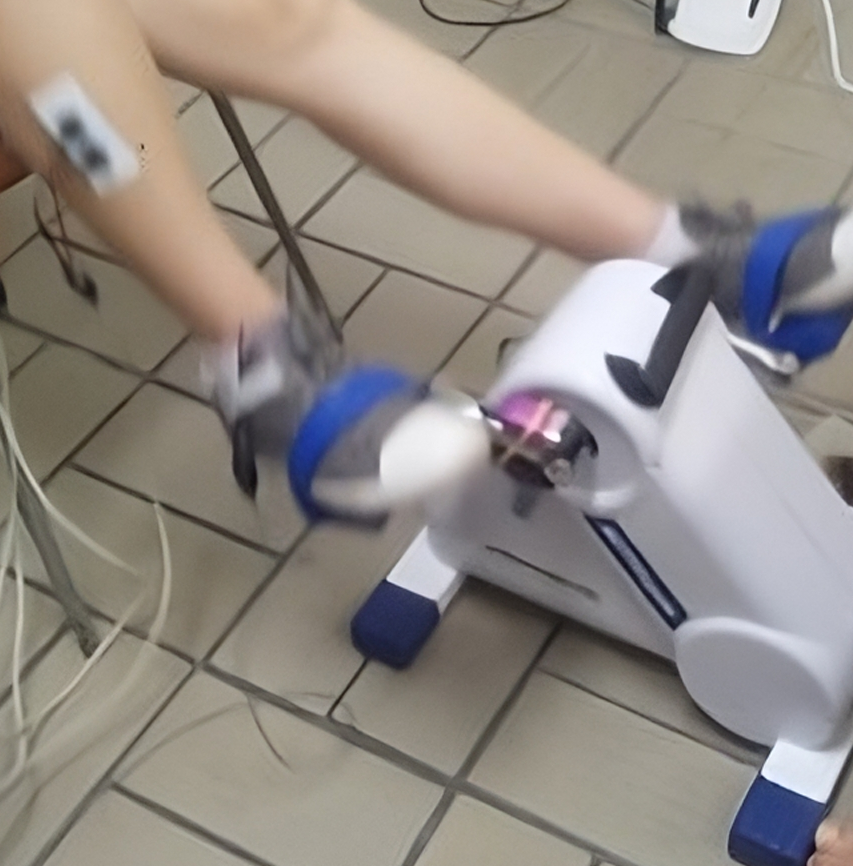
\includegraphics[scale=0.2]{images/sa.png}
    \caption{Sistema de adquisición de datos}
    \label{fig: sa}
\end{figure}    

El funcionamiento del videojuego se logra por medio de dos componentes del pedal:
\begin{itemize}
    \item El primer componente (sensor óptico) controla la velocidad de movimiento en el videojuego, por  medio de la acción de pedaleo del paciente en rehabilitación. A medida que se logra una velocidad definida, se envía la orden de movimiento al videojuego y este responde con el movimiento del avatar en la escena, el cual se encuentra en una pista cuyo objetivo será alcanzar los mejores resultados de tiempo, distancia o  MCV(Máxima contracción voluntaria).
    \item El segundo componente del sistema (sensores de EMG) tienen la función de capturar la señal EMG obtenida en la una rutina de entrenamiento y ser usados tanto en la dificultad de los niveles de entrenamiento de la rutina clínica como para la estadística de la misma.
\end{itemize}
    
Dichos componentes, tanto internos como externos, se encuentran orientados hacia  la realización de un objetivo común: el desarrollo de la capacidad física tanto para usuarios sanos como enfermos. A continuación se presentan las características funcionales del sistema, (ver figura~\ref{fig: system}):

\vspace{5pt}
La aplicación de juego serio es responsable de:
\begin{itemize}
    \item Recibir y procesar las señales de la plataforma Arduino incluido en el pedal para ser utilizadas tanto en la animación de la escena como en la estadística.
    \item La carga y procesamiento de las escenas y los paradigmas de las rutinas junto a la lógica asociada. 
    \item Procesar los eventos registrados durante la realización de la rutina y devolver un análisis sobre los resultados.
    \item Gestionar los datos del usuario.
\end{itemize}

\vspace{5pt}
El pedal motorizado es responsable de:
\begin{itemize}
    \item Registrar a partir de electrodos las señales EMG del cuerpo humano correspondientes al tren inferior.
    \item Registrar la velocidad angular en los pedales.
    \item Enviar en tiempo real los datos registrados a cualquier aplicación de juego serio sincronizada.
\end{itemize}
    
\begin{figure}[ht]
    \centering
    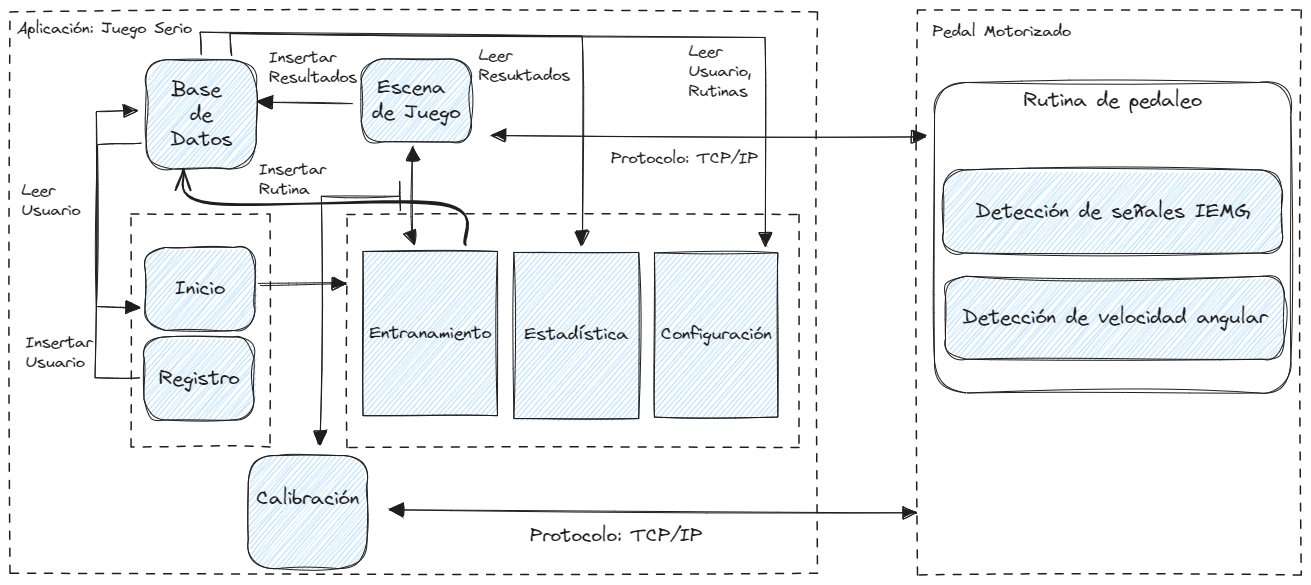
\includegraphics[scale=0.3]{images/system.png}
    \caption{Diagrama del sistema}
    \label{fig: system}
\end{figure}